\titre{Modèle} : Une représentation du monde réel. En physique et en maths, il prend ses valeurs dans des espaces denses, en informatique dans des espaces discrets finis.\\

\titre{Problème/Algorithme/Programme} Ne pas confondre les 3 notions.\\

\titre{Problème} : Du grec problema (jeté devant ie obstacle). Un problème est constitué d'une situation initiale et d'un but à atteindre pour la situation finale.

\titre{Algorithme} : (Al Khwarizmi : 820 ap JC) Une façon systématique de procéder pour faire quelque chose en un nombre fini d'étapes élémentaires.\\

\titre{Programme} : Mise en oeuvre concrète d'un algorithme dans un langage de programmation.\\
   
\titre{Preuve de programme} : On peut prouver qu'il y a conformité entre le modèle mathématique et le programme, mais pas qu'il répond à la sémantique naturelle du problème (ie qu'il marche). Il faudrait pour cela être capable de tester TOUS les cas possibles.\\

\titre{Syntaxe/Sémantique} : La syntaxe est maîtrisable, mais pas la sémantique.\\

\titre{Ambiguité} : Les langages naturels sont ambigus ("Rogrigue, as tu du coeur?"), tandis que les langages de programmation ne le sont pas $\impl$ déterminisme.\\

\titre{Compilateur} : \begin{enumerate}
	\item \titre{parsing} ou \titre{analyse lexicale} : Assemble les symboles en groupes formant des expressions. 
	\item \titre{analyse syntaxique} : Vérifie que les expressions sont grammaticalement correctes.
	\item \titre{table des symboles} : Visibilité des symboles, renommage, contrôle de type.
	\item \titre{génération de code} : syntaxe abstraite.
\end{enumerate}

\titre{Abstrait} : En informatique, abstrait signifie : on oublie certaines informations.  

\titre{Grammaire regex} : Fait elle partie des grammaires hors contexte ? (oui ?)

\newpage

\titre{Grammaire hors contexte} : Ne dépend pas du contexte. Elle est constituée de : 
\begin{itemize}
	\item Un ensemble $T$ de symboles terminaux (alphabet des symboles)
	\item Un ensemble $N$ de symboles non-terminaux ($T\cap N =\vide$) (alphabet des variables -> à voir comme une catégorie.
	\item Un ensemble $R$ de règles (couples $(x,y)$ notés $x \rightarrow y$, de mots sur $V\cup N$) 
	\item Un symbole de départ $S\in N$
\end{itemize}

\titre{Exemple} : Un entier 
\begin{itemize}
	\item $T = \{-,0,1,2,3,4,5,6,7,8,9\}$
	\item $N = \{<chiffre>,<entier>,<suite>\}$
	\item Règles : \begin{itemize}
		\item $<entier> ::= (-|\varepsilon) <origine><suite>$ 
		\item $<suite> ::= (0|<chiffre>)<suite> | \varepsilon$
		\item $<chiffre> ::= 1|2|3|4|5|6|7|8|9$
		\end{itemize}
	\item $S = <entier>?$
\end{itemize}
Construction de l'arbre de $243$ :\\
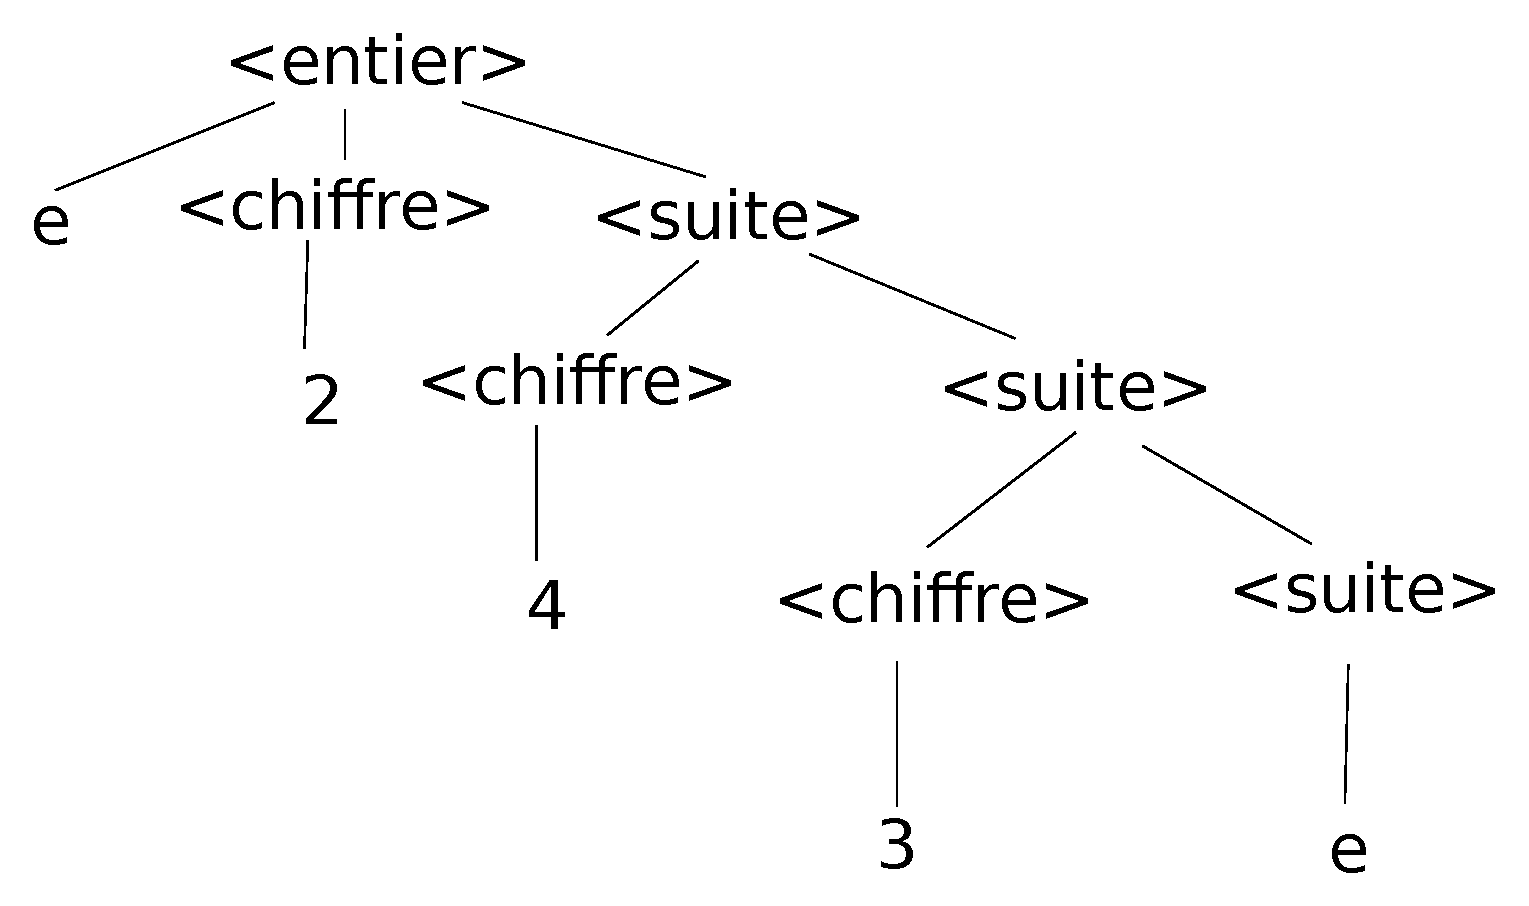
\includegraphics[width=\linewidth]{fig1_graphe_BNF_entier.pdf}


